\chapter{Fitness Dynamics}
\section{Θεωρητική Ανάλυση του Fitness Dynamics}
Σε αυτό το σημείο θα αναλύσουμε την  \nameref{appendix:TourTF} .



Τα ορίσματα όπως ζητάει η εκφώνηση είναι το B ο πίνακας του παίγνιου, το Strategies που είναι διάνυσμα \texttt{strings} με τις στρατηγικές και συμπληρώνεται από το \texttt{Pop0} το οποίο είναι ο αρχικός πλυθησμός που παρευρίσκεται στο παιχνίδι. Το \( Τ\) ο αριθμός των γύρων και το \(J\) ο αριθμός των γενεών που θα τρέχει το πρωτάθλημα.
Αρχικά λαμβάνουμε τον πίνακα \texttt{Re\_matrix} (από τη συνάρτηση \nameref{appendix:RewST} ) ο οποίος είναι ο πίνακας των Scores μετά από έναν συγκεκριμένο αριθμό γύρων. 
\\

Η συνάρτηση αυτή υλοποιεί ένα παιχνίδι Axel \(Τ\) γύρων και επιστρέφει τον πίνακα με τα scores μεταξύ των στρατηγικών. 
Στη συνέχεια, λαμβάνουμε στην μεταβλητή \(P\) το άθροισμα των πληθυσμών στις στρατηγικές που παίζουμε δηλαδή τον αρχικό συνολικό πληθυσμό και αρχικοποιούμε τις μεταβλητές επιστροφής.
\\

 To \texttt{POP} επιστρέφει τις τιμές του πληθυσμού ανά γενιά, το \texttt{BST} τις βέλτιστες στρατηγικές ανα γενιά ενώ το \texttt{FIT} το fitness των στρατηγικών. Στη συνέχεια αναθέτουμε τον αρχικό πληθυσμό στην πρώτη θέση του array του \texttt{POP} και υπολογίζουμε το fitness της κάθε στρατηγικής δηλαδή το άθροισμα των score επί τον πλυθησμό με βάση τη συγκεκριμένη στρατηγική αφαιρώντας τις περιπτώσεις που οι στρατηγικές παίζουν με τον εαυτό τους όπως αναλύεται και στο paper\cite{paper}.
\\

Στη συνέχεια υπολογίζονται οι συνολικοί πόντοι \(t\) που έχουν δοθεί σε όλες τις στρατηγικές και ψάχνουμε να βρούμε αυτές με το βέλτιστο fitness για την έξοδο του \texttt{BST}.
\\
Ο πληθυσμός ανανεώνεται με βάση τους τύπους του paper\cite{paper}: \begin{align*}
W_{n+1}(A) &= \frac{\Pi W_n(A) g_n(A)}{t(n)} \\
W_{n+1}(B) &= \frac{\Pi W_n(B) g_n(B)}{t(n)} \\
W_{n+1}(C) &= \frac{\Pi W_n(C) g_n(C)}{t(n)}
\end{align*} και το ερώτημα που γεννάται είναι κατά πόσο η ανάλυση αυτή είναι σωστή με την παραδοχή ότι δεν γίνεται στρογγυλοποίηση και το \texttt{POP} διάνυσμα περιέχει πραγματικές τιμές.
Για τον σκοπό αυτό προσθέτουμε την προτροπή του paper σύμφωνα με το οποίο οι πληθυσμοί της επόμενης γενιάς υπλογίζονται από το floor της κάθε παράστασης.
Εδώ πέρα γεννάται το ερώτημα εάν το συγκεκριμένο «επιπόλαιο» rounding κρατήσει ίδιο τον συνολικό πληθυσμό και με την πρώτη δοκιμή παρατηρούμε ότι δεν τον κρατάει. Συνεπώς πρέπει να αποφασίσουμε αν θα χρησιμοποιήσουμε τον ίδιο πληθυσμό με τον αρχικό ή κάθε φορά θα τον ξαναμετράμε για να συμπεριλάβουμε το σφάλμα του rounding. Ωστόσο στη δεύτερη περίπτωση παρατηρούμε το σφάλμα ανά γενιά να συσσωρεύεται οδηγώντας στην κατάρρευση του συστήματος. 
Συνεπώς η υλοποίηση η οποία ακολουθεί πιστά και το paper είναι να μετρήσουμε μια φορά τον συνολικό πληθυσμό και σε κάθε γενιά να χρησιμοποιούμε αυτή τη σταθερή τιμή \(P \) κάνοντας floor rounding ακόμα και αν αυτό οδηγήσει στο τέλος σε μια μικρή απώλεια.
Τα αποτελέσματα που παρήχθησαν μπορούν να φανούν παρακάτω:
\begin{figure}[htbp]
\vspace*{1em}
  \centering
  \begin{minipage}{0.48\textwidth}
    \centering
 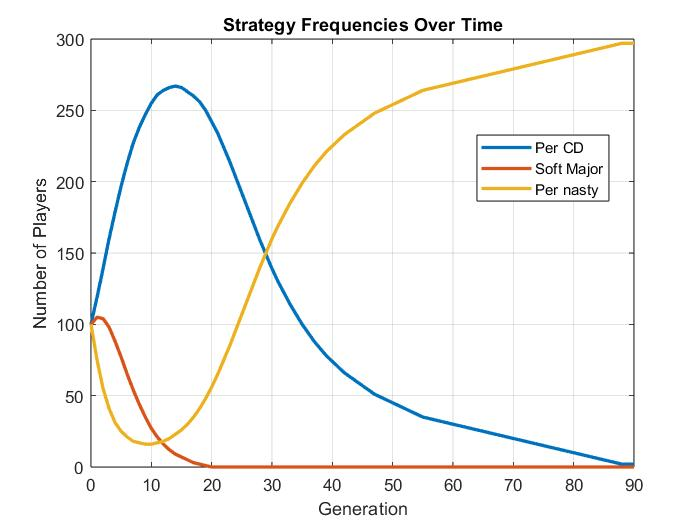
\includegraphics[width=0.8\linewidth]{fit_plots_theoretical/defectors_may_be_strong}

\label{fig:defectorsmaybestrong}
  \end{minipage}
  \hfill
  \begin{minipage}{0.48\textwidth}
    \centering
  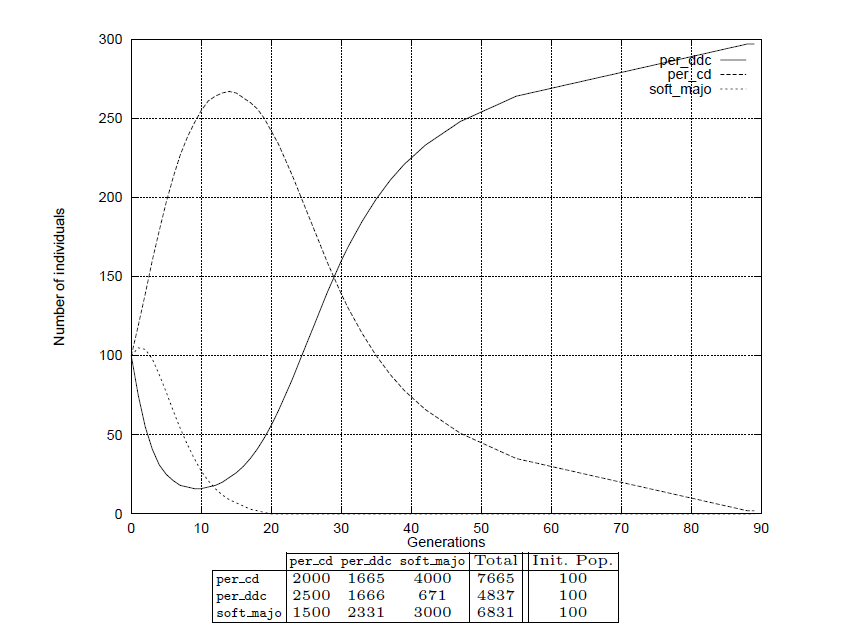
\includegraphics[width=0.8\linewidth]{defectors_may_be_strong }

  \end{minipage}
  \caption{Defectors may be Strong (\texttt{defectors\_may\_be\_strong.m})}
\end{figure}

\begin{figure}[htbp]
  \centering
  \begin{minipage}{0.48\textwidth}
    \centering
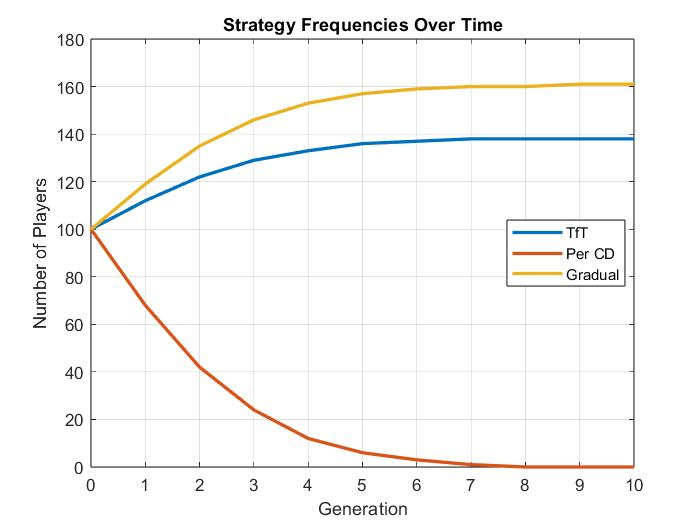
\includegraphics[width=0.8\linewidth]{fit_plots_theoretical/monotonous_convergence}

  \end{minipage}
  \hfill
  \begin{minipage}{0.48\textwidth}
    \centering
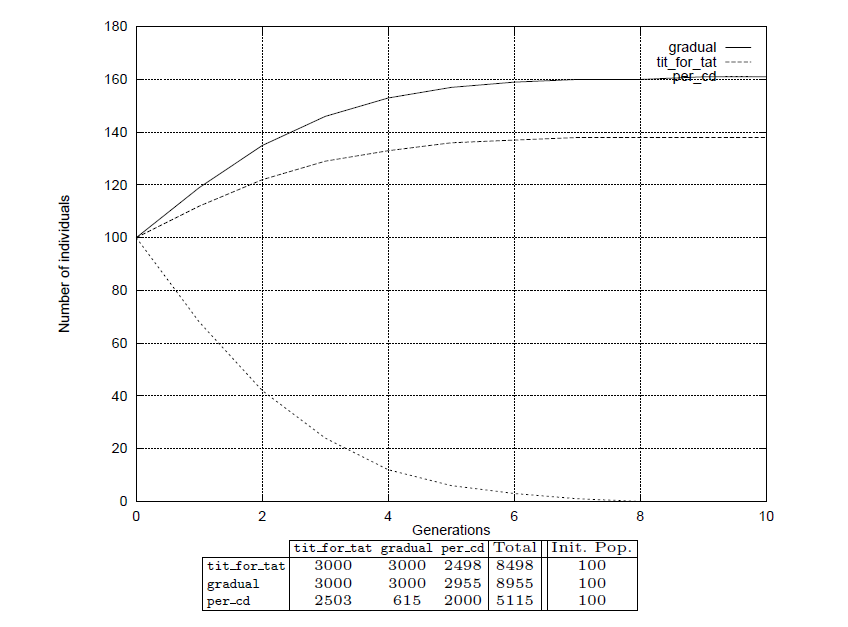
\includegraphics[width=0.8\linewidth]{monotonous_convergence}

  \end{minipage}\caption{Monotonous Convergence (\texttt{monotonous\_convergence.m})}
\end{figure}

\begin{figure}[htbp]
	\centering
	\begin{minipage}{0.48\textwidth}
		\centering
		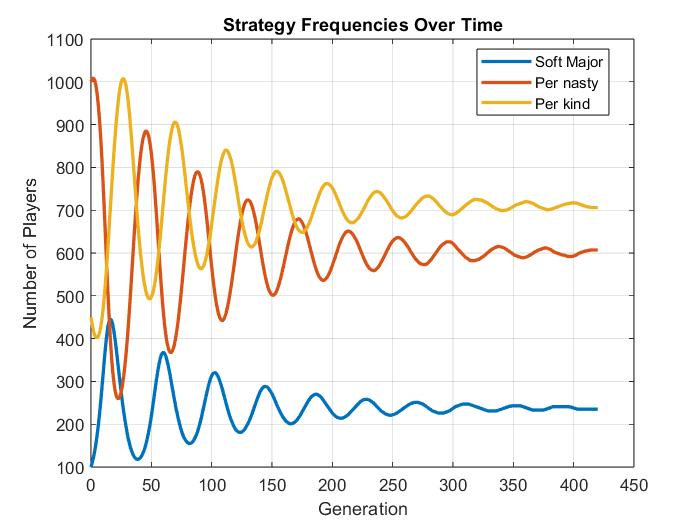
\includegraphics[width=0.8\linewidth]{fit_plots_theoretical/attenuated_oscillatory_movements}
	
	\end{minipage}
	\hfill
	\begin{minipage}{0.48\textwidth}
		\centering
		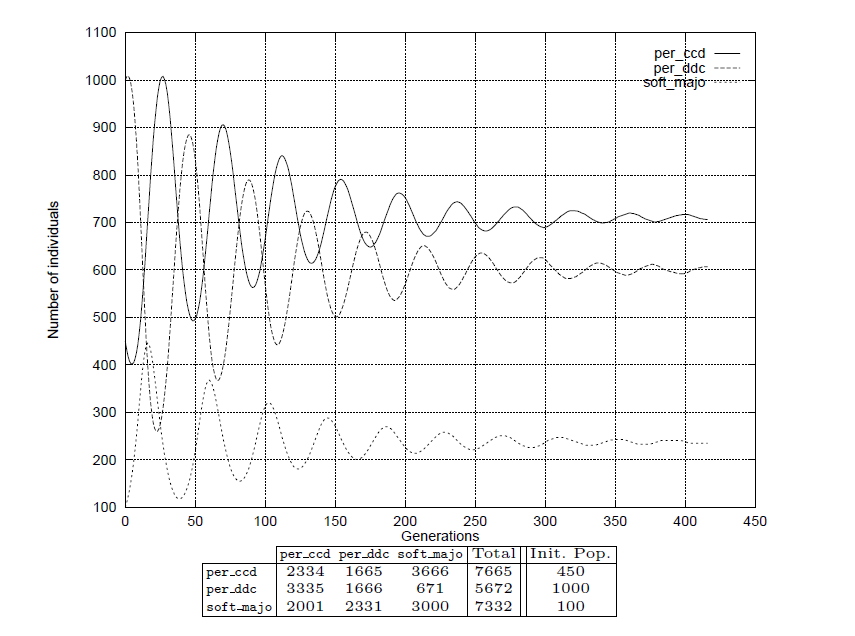
\includegraphics[width=0.8\linewidth]{attenuated_oscillatory_movements}
	
	\end{minipage}
		\caption{Attenuated\_oscillatory\_movements (\texttt{attenuated\_oscillatory\_movements.m})}

\end{figure}
\clearpage





% TODO: \usepackage{graphicx} required
\begin{figure}[ht!]
\centering
	\begin{minipage}{0.48\textwidth}
	\includegraphics[width=1\linewidth]{fit_plots_theoretical/Increasing_Oscillations}

	
	\end{minipage}
	\begin{minipage}{0.48\textwidth}
		\includegraphics[width=1\linewidth]{Increasing_Oscillations}
	\end{minipage}
	\caption{Increasing Oscillations (\texttt{increasing\_oscillations.m})}
\end{figure}

\begin{figure}[ht!]
	\centering
	\begin{minipage}{0.48\textwidth}
		\includegraphics[width=1\linewidth]{fit_plots_theoretical/Periodic_Movements}
		
		
	\end{minipage}
	\begin{minipage}{0.48\textwidth}
		\includegraphics[width=1\linewidth]{Periodic_Movements}
	\end{minipage}
	\caption{Periodic Movements \texttt{(periodic\_movements.m)}}
\end{figure}

\begin{figure}[ht!]
	\centering
	\begin{minipage}{0.48\textwidth}
		\includegraphics[width=1\linewidth]{fit_plots_theoretical/Disordered_Oscillations}
		
		
	\end{minipage}
	\begin{minipage}{0.48\textwidth}
		\includegraphics[width=1\linewidth]{Disordered_Oscillations}
	\end{minipage}
	\caption{Disordered Oscillations \texttt{(Disordered Oscillations.m)}}
\end{figure}

\begin{figure}[ht!]
	\centering
	\begin{minipage}{1\textwidth}
		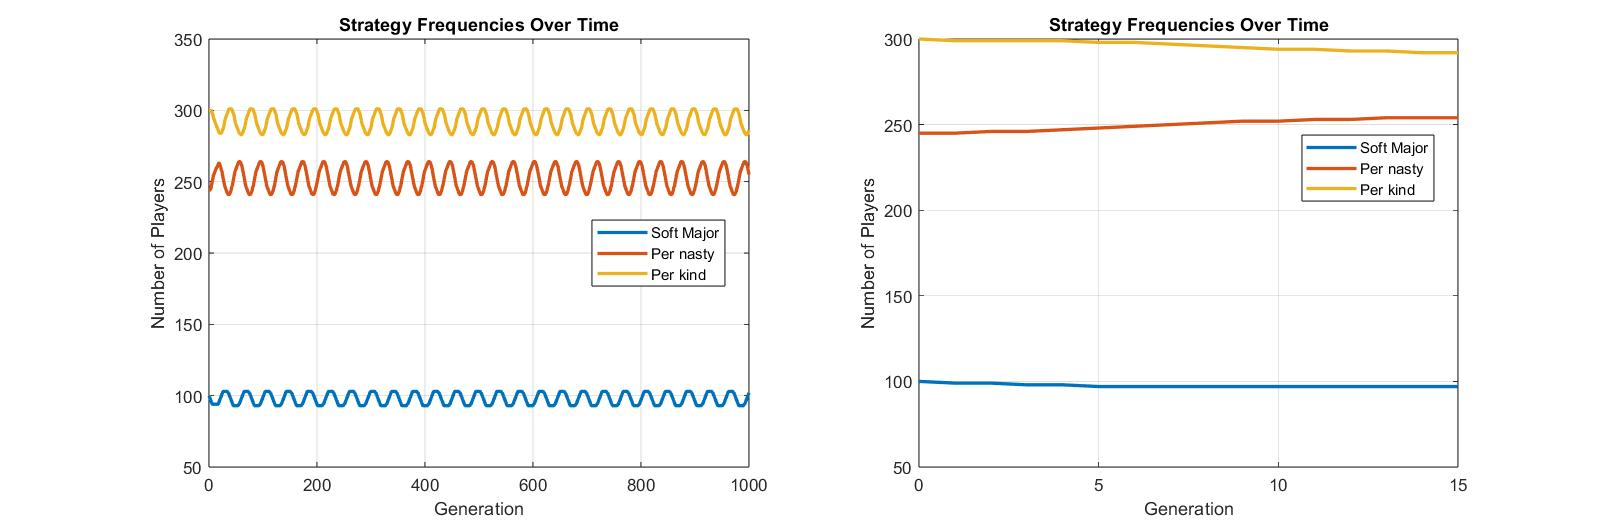
\includegraphics[width=1\linewidth]{fit_plots_theoretical/sensitivity_to_population_size}
		
		
	\end{minipage}
	\begin{minipage}{1\textwidth}
		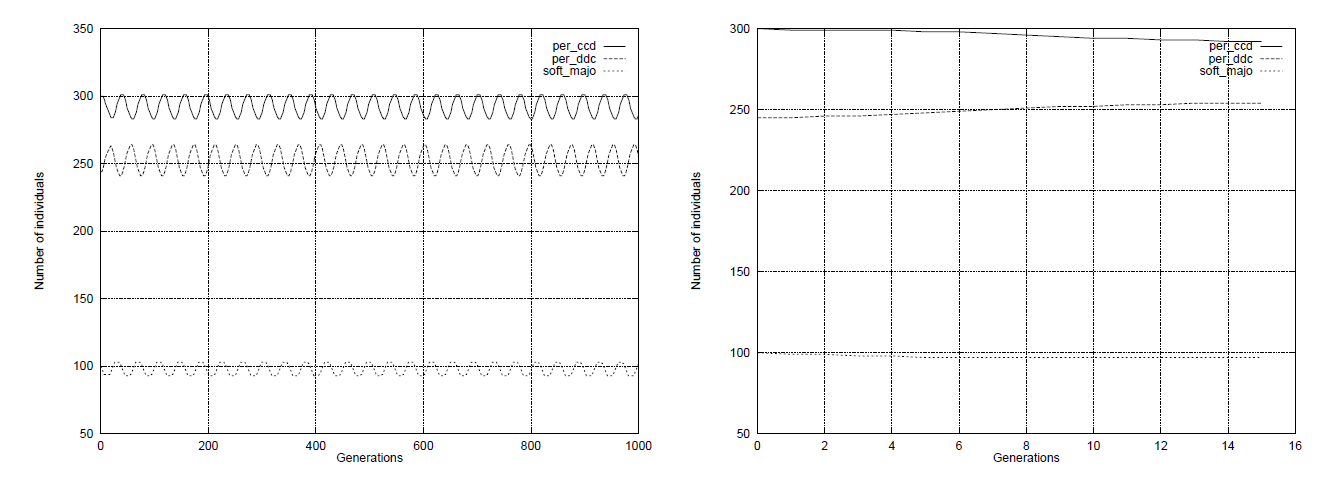
\includegraphics[width=1\linewidth]{sens_popsize}
	\end{minipage}
	\caption{Sensitivity of dynamics to population's size. All parameters are identical except
		for the initial size of per ddc which is 244 on the left and 245 on the right \texttt{(sens\_dyn\_pop\_size.m)}}
\end{figure}

\begin{figure}[ht!]
	\centering
	\begin{minipage}{1\textwidth}
		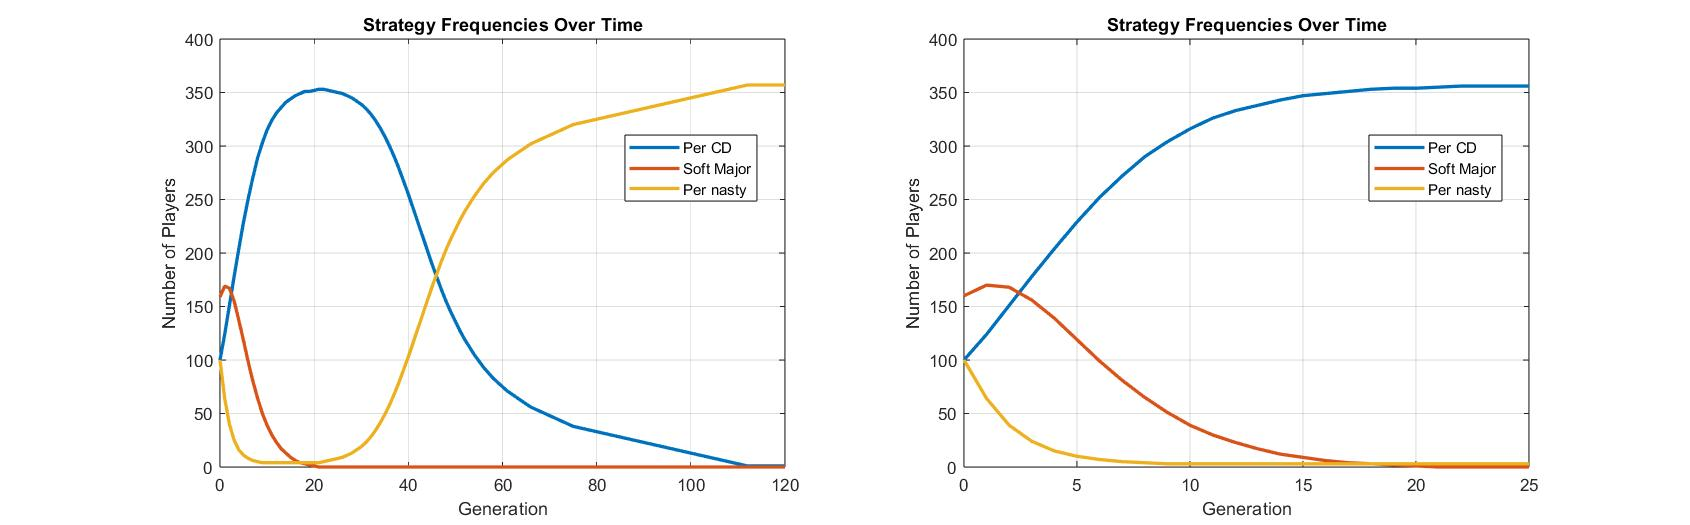
\includegraphics[width=1\linewidth]{fit_plots_theoretical/sensitivity_of_winner_to_popsize}
		
		
	\end{minipage}
	\begin{minipage}{1\textwidth}
		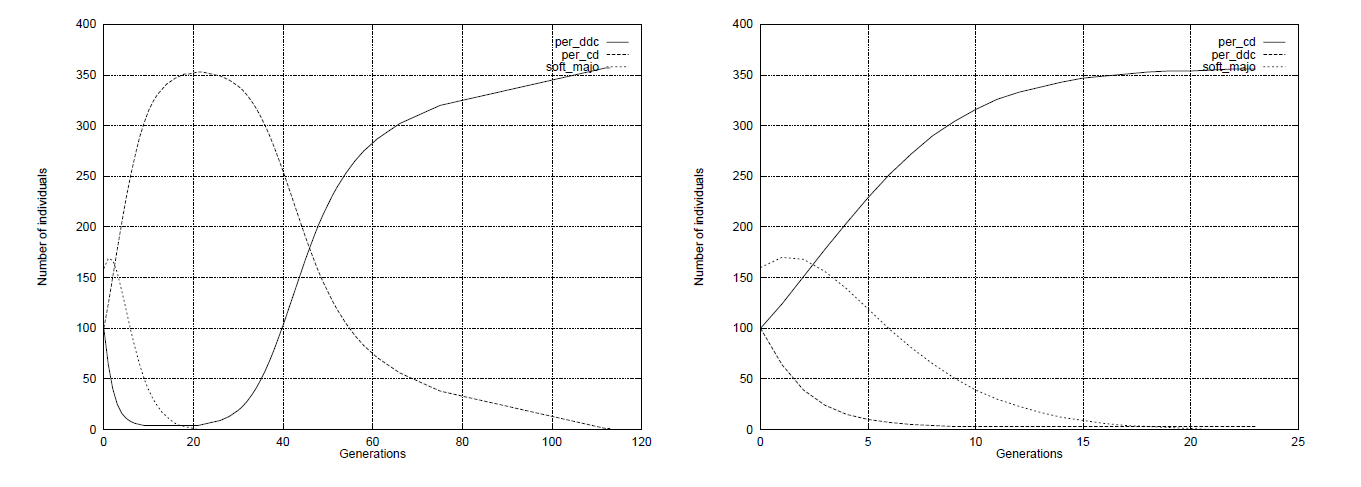
\includegraphics[width=1\linewidth]{sens_winner}
	\end{minipage}
	\caption{Sensitivity of winner to population's size. All parameters are identical except
		for the initial size of soft majo which is 159 on the left and 160 on the right.(\texttt{sens\_win\_pop\_size.m})}
\end{figure}

\begin{figure}[ht!]
	\centering
	\begin{minipage}{1\textwidth}
		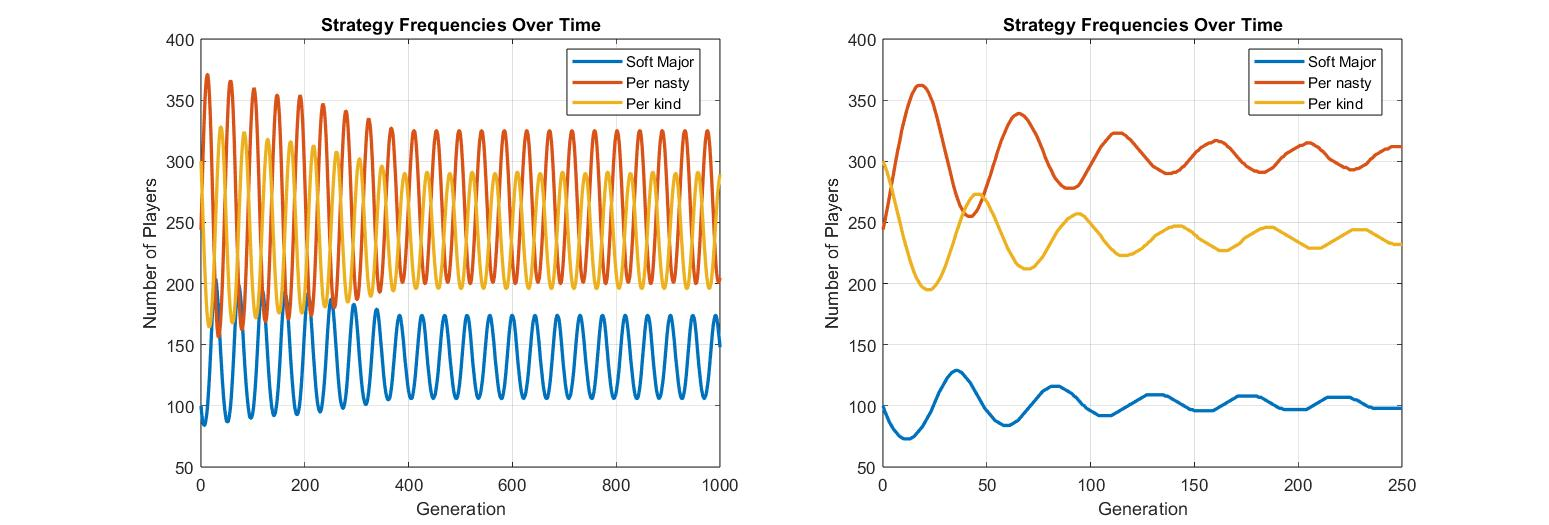
\includegraphics[width=1\linewidth]{fit_plots_theoretical/sensitivity_to_game_length}
		
		
	\end{minipage}
	\begin{minipage}{1\textwidth}
		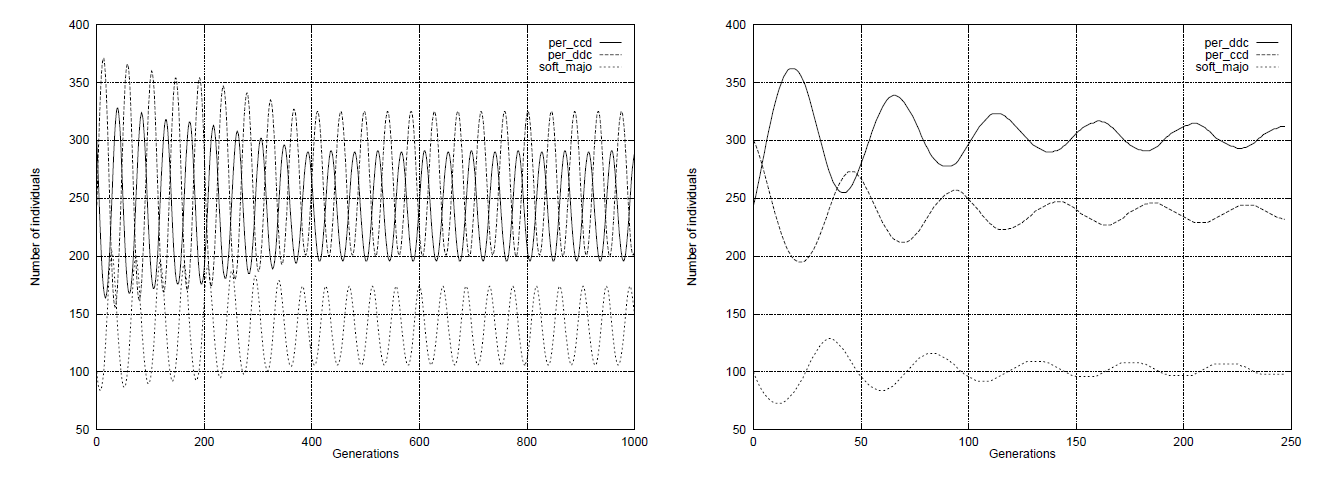
\includegraphics[width=1\linewidth]{sens_gamelength}
	\end{minipage}
	\caption{Sensitivity to game length. All parameters are identical except for the game
	length which is 7 moves on the left and 6 on the right \texttt{(sens\_game\_length.m)}}
\end{figure}


\begin{figure}[ht!]
	\centering
	\begin{minipage}{1\textwidth}
		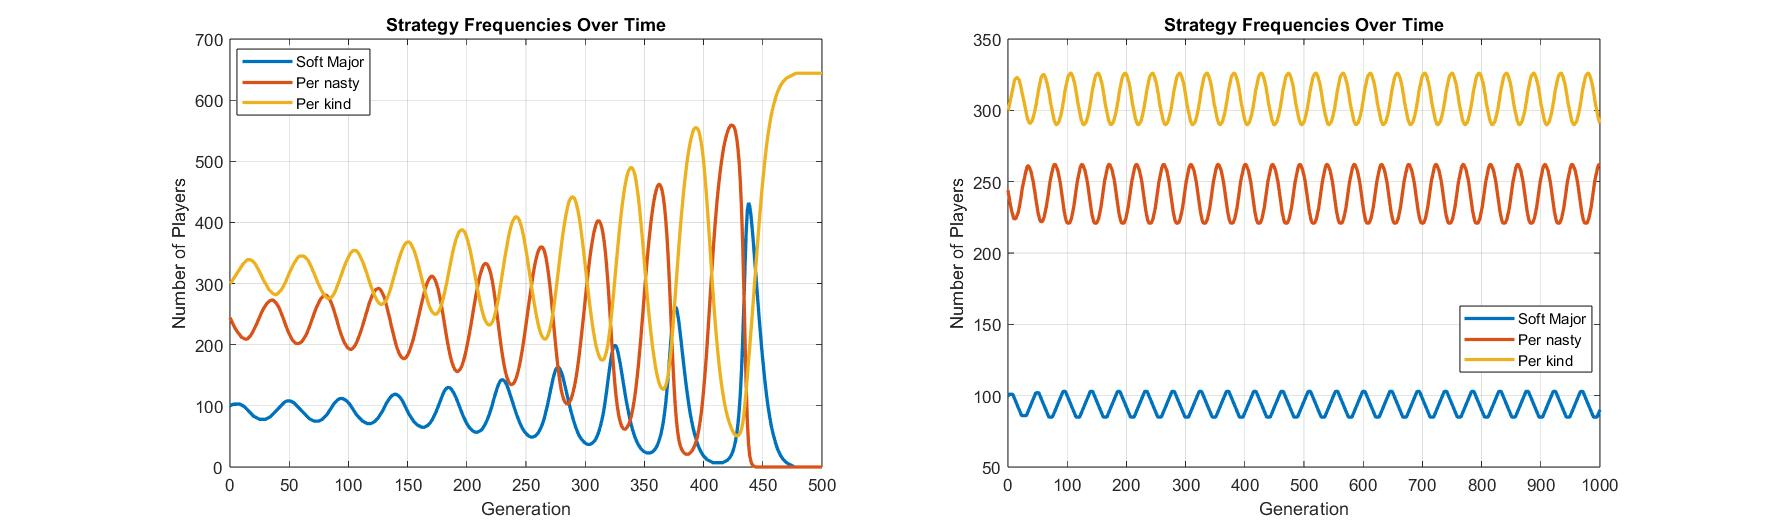
\includegraphics[width=1\linewidth]{fit_plots_theoretical/sensitivity_to_cipd_payoff}
		
		
	\end{minipage}
	\begin{minipage}{1\textwidth}
		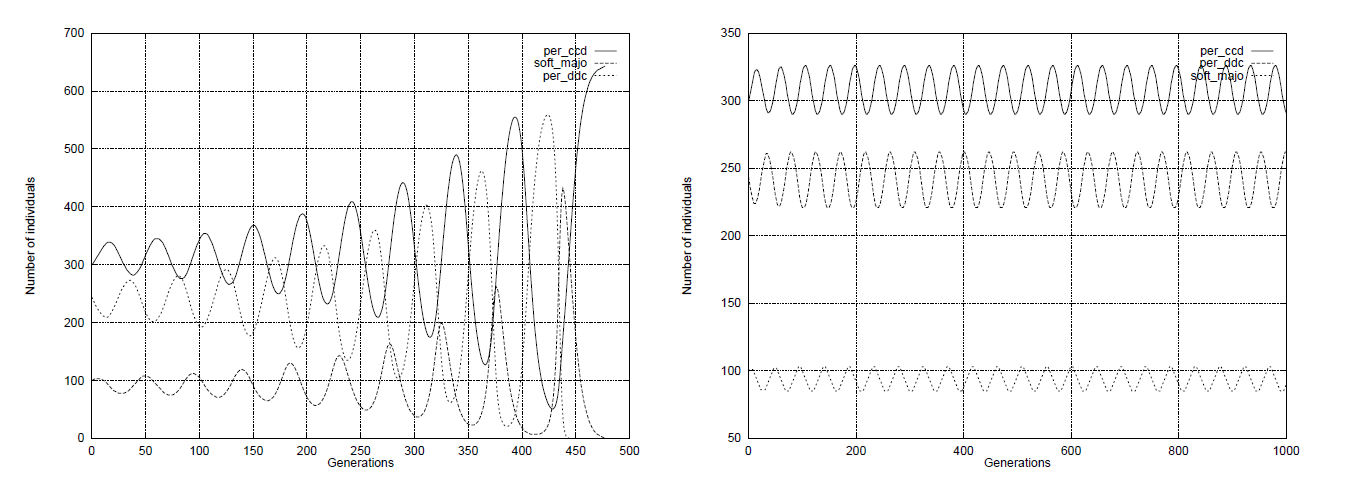
\includegraphics[width=1\linewidth]{sens_cipd}
	\end{minipage}
	\caption{Sensitivity to CIPD payoff. All parameters are identical except that \(T=4.6\)
		on the left and \( T=4.7\) on the right. (\texttt{sens\_cipd\_payoff.m})}
\end{figure}

\begin{figure}[ht!]
	\centering
	\begin{minipage}{1\textwidth}
		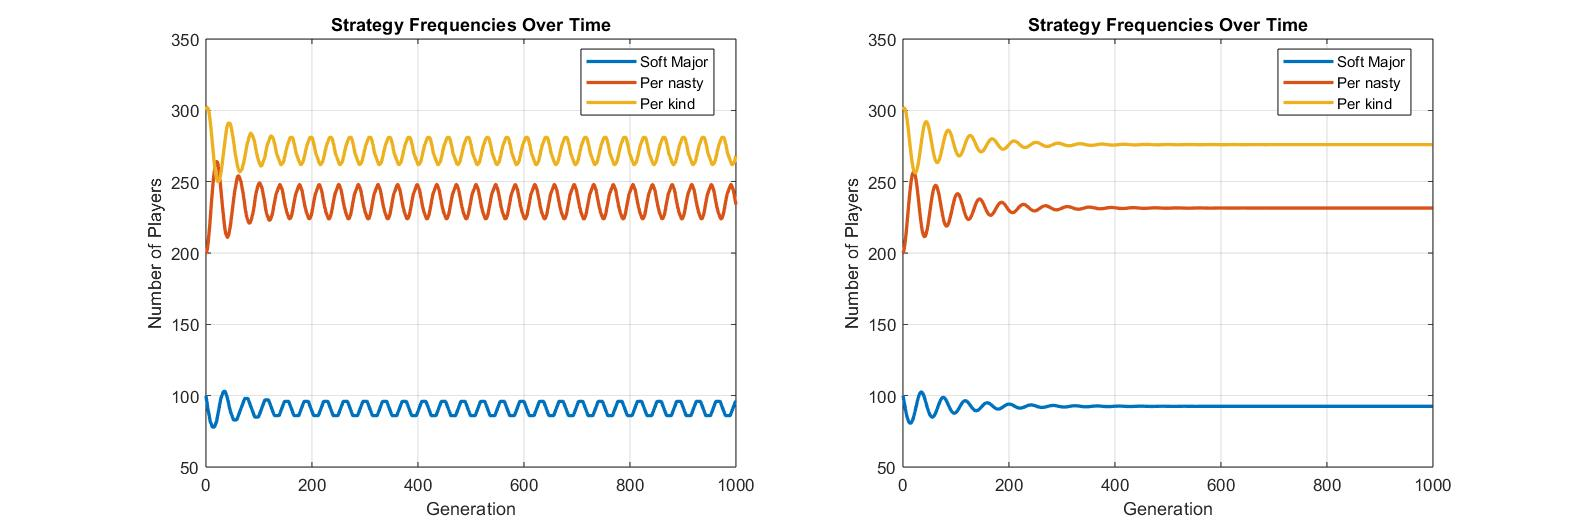
\includegraphics[width=1\linewidth]{fit_plots_theoretical/repartition_real}
		
		
	\end{minipage}
	\begin{minipage}{1\textwidth}
		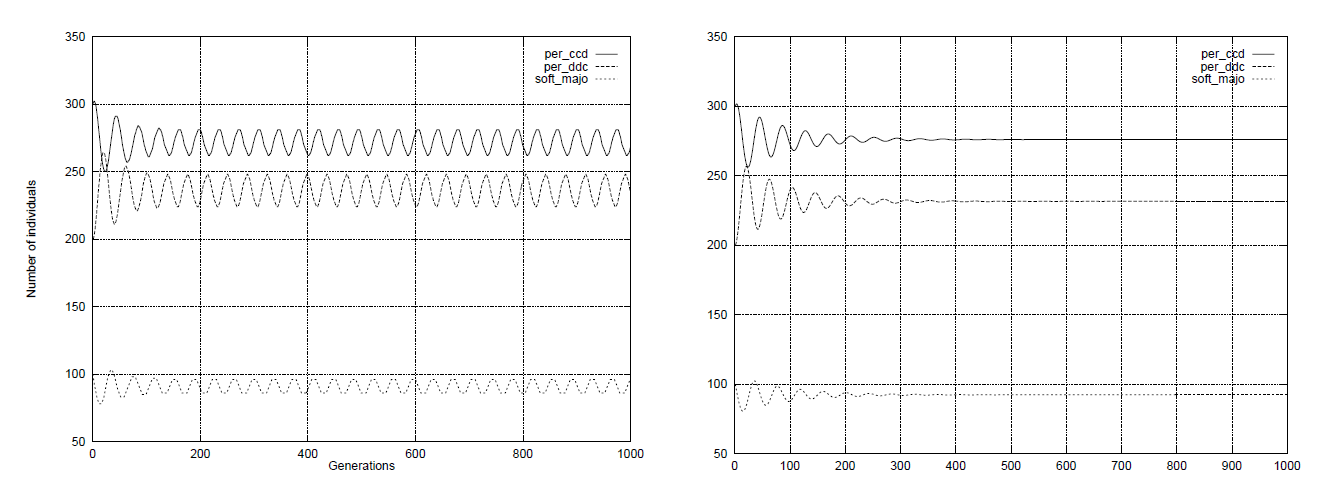
\includegraphics[width=1\linewidth]{sens_real}
	\end{minipage}
	\caption{Sensitivity to repartition computation method. All parameters are identical
		except that repartition on the left is done by rounding and uses real value on the right. (\texttt{sens\_repartition\_real.m})}
\end{figure}

\begin{figure}[ht!]
	\centering
	\begin{minipage}{1\textwidth}
		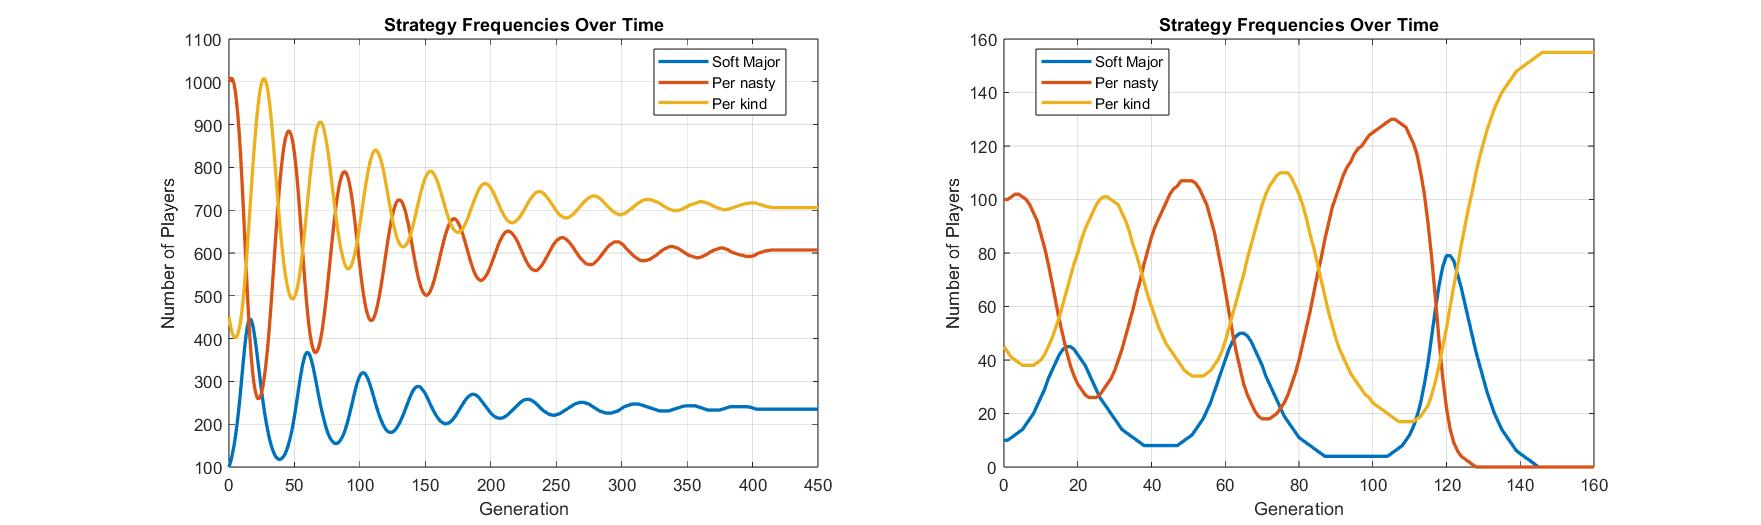
\includegraphics[width=1\linewidth]{fit_plots_theoretical/repartition_div10}
		
		
	\end{minipage}
	\begin{minipage}{1\textwidth}
		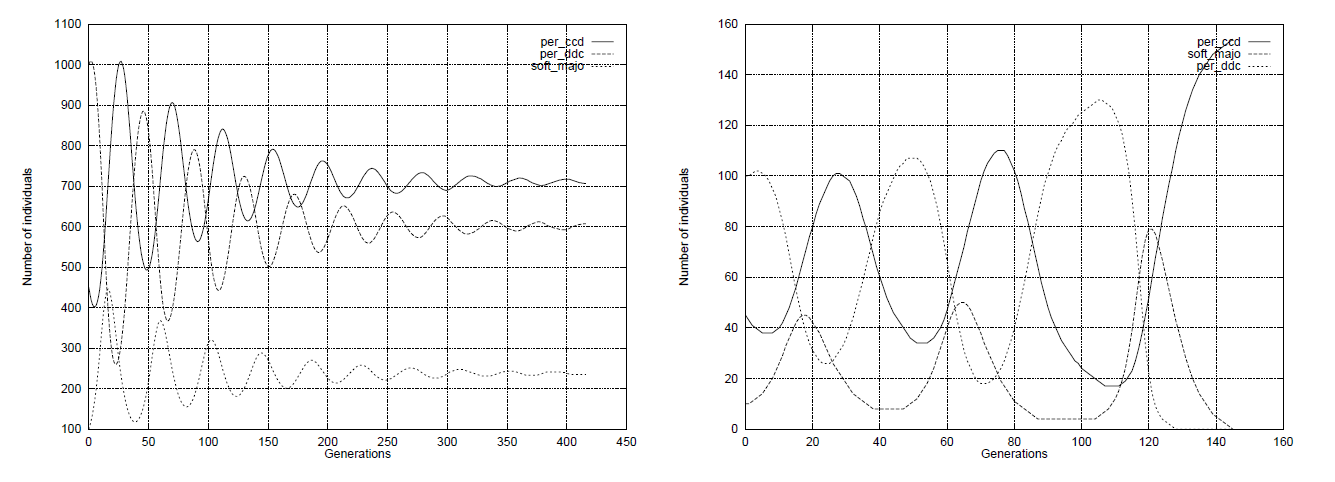
\includegraphics[width=1\linewidth]{sens_div10}
	\end{minipage}
	\caption{Sensitivity to repartition computation method. All parameters are identical
		except that populations on the right are divided by 10. (\texttt{sens\_repartition\_div10.m})}
\end{figure}


\clearpage

Παρατηρούμε την επ’ ακριβώς αντιστοίχιση με τα αποτελέσματα του paper ακόμα και σε επίπεδο debugging βλέποντας τους πίνακες των κερδών.
Στη συνέχεια επιχειρήσαμε να δημιουργήσουμε αυτές τις καμπύλες τρέχοντας προσομοιώσεις όπου είχαμε να αποφασίσουμε μεταξύ της πλήρους ή της μερικής προσομοίωσης.

\section{Προσομοίωση του Fitness Dynamics}
Στη συνέχεια επιχειρήσαμε να δημιουργήσουμε αυτές τις καμπύλες τρέχοντας προσομοιώσεις όπου είχαμε να αποφασίσουμε μεταξύ της πλήρους ή της μερικής προσομοίωσης.
Για τους σκοπούς αυτούς χρησιμοποιούμε τη συνάρτηση \nameref{appendix:TSF} η οποία αναλύεται παρακάτω:
\subsection{Θεωρητική Αναλυση του TourSimFit:
}




Η συνάρτηση αυτή είναι παρόμοια με την \texttt{TourTheFit} . Η βασική διαφορά είναι ότι για να διατηρηθεί ο πληθυσμός με ακέραιες τιμές χρησιμοποιούμε την συνάρτηση \nameref{appendix:CIV}


Η συνάρτηση αυτή ουσιαστικά μεταφέρει το περισσευούμενο fractional part στα στοιχεία με το χαμηλότερο fractional part. 
\\
\\
Σημαντική διαφορά εδώ είναι ότι , για να έχουμε μεγαλύτερη ταχύτητα στο Simulation, εκτελούμε τον κώδικα χρησιμοποιώντας την συνάρτηση \nameref{appendix:A2I}.
\\

Έτσι εκτελούμε μια μορφή half simulation (όχι καθαρή προσομοίωση). 
\\

Τρέχοντας ξανά τις παρακάτω προσομοιώσεις παρατηρούμε τα εξής για το κάθε ένα πείραμα.
\subsubsection{Defectors may be strong}

% TODO: \usepackage{graphicx} required
\begin{figure}[ht!]
\centering
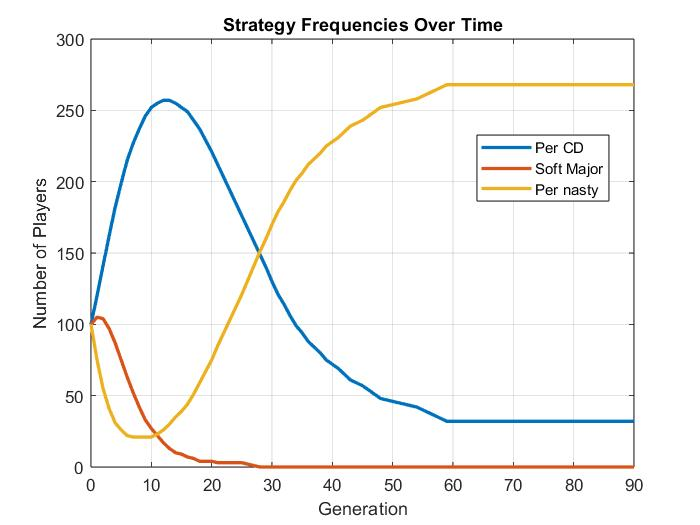
\includegraphics[width=0.5\linewidth]{fit_plots_simulations/defectors_may_be_strong_sim}
\caption{\texttt{defectors\_may\_be\_strong\_sim.m}}
\label{fig:defectorsmaybestrongsim}
\end{figure}

Παρατηρούμε παρόμοια συμπεριφορά με ίδιες γραφικές παραστάσεις με τη μόνη διαφορά η προσομοίωση να οδηγείται σε steady state μερικές γενιές νωρίτερα
\clearpage

\subsubsection{Monotonous Convergence}
% TODO: \usepackage{graphicx} required
\begin{figure}[th!]
\centering
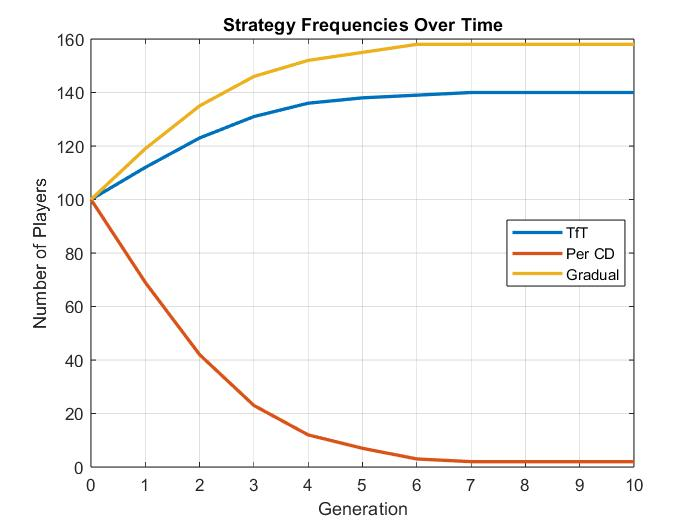
\includegraphics[width=0.7\linewidth]{fit_plots_simulations/monotonous_convergence_sim}
\caption{\texttt{monotonous\_convergence\_sim.m}}
\label{fig:monotonousconvergencesim}
\end{figure}

Παρατηρούμε και εδώ παρόμοια συμπεριφορά με ίδιες γραφικές παραστάσεις και ελαφρά αλλαγμένους τους πληθυσμούς του steady state.


\subsubsection{Attenuated Oscillations}
% TODO: \usepackage{graphicx} required
\begin{figure}[th!]
\centering
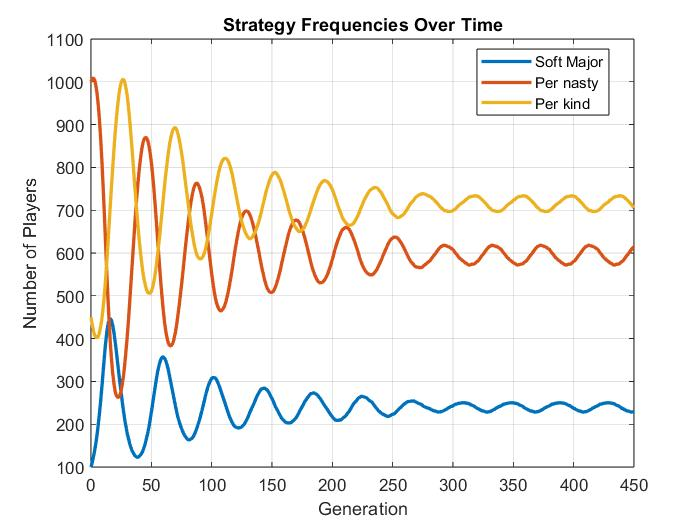
\includegraphics[width=0.7\linewidth]{fit_plots_simulations/attenuated_oscillatory_movements_sim}
\caption{\texttt{attenuated\_oscillatory\_movements\_sim.m}}
\label{fig:attenuatedoscillatorymovementssim}
\end{figure}

Παρατηρούμε παρόμοια συμπεριφορά με ίδιες γραφικές παραστάσεις με το simulation να έχει μικρότερο βαθμό απόσβεσης.


\subsubsection{Periodic Movements}
% TODO: \usepackage{graphicx} required
\begin{figure}[th!]
\centering
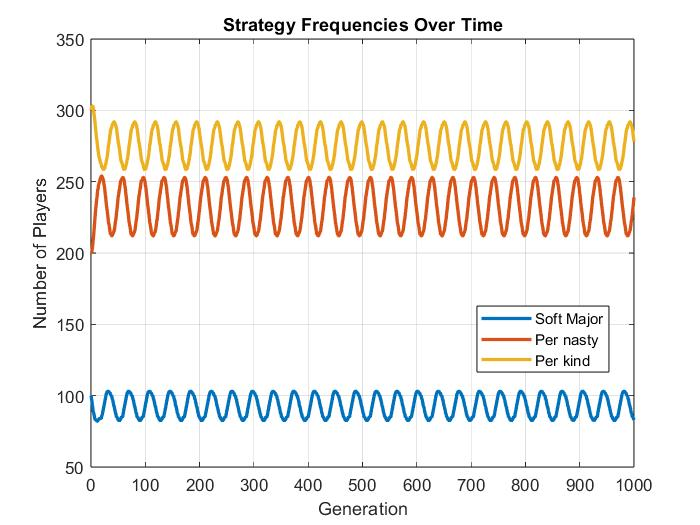
\includegraphics[width=0.7\linewidth]{fit_plots_simulations/periodic_movements_sim}
\caption{\texttt{periodic\_movements\_sim.m}}
\label{fig:periodicmovementssim}
\end{figure}

Παρατηρούμε παρόμοια συμπεριφορά με τη θεωρητική ανάλυση
\subsubsection{Increasing Oscillations}
% TODO: \usepackage{graphicx} required
\begin{figure}[th!]
\centering
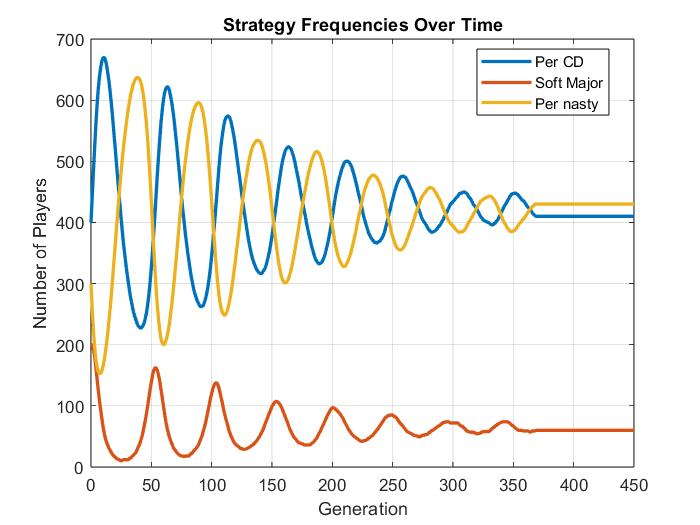
\includegraphics[width=0.7\linewidth]{fit_plots_simulations/increasing_oscillations_sim}
\caption{\texttt{increasing\_oscillations\_sim.m}}
\label{fig:increasingoscillationssim}
\end{figure}

Παρατηρούμε σημαντική διαφορά καθώς στην περίπτωση της προσομοίωσης δε συμβαίνουν αυξανόμενες ταλαντώσεις. Αυτό οφείλεται στον τρόπο που γίνεται το rounding στην προσομοίωση και εμφανίζεται και σε επόμενα πειράματα πολλές φορές χαλώντας και την κατάταξη των στρατηγικών. Στο συγκεκριμένο αν και οι ταλαντώσεις είναι μειούμενες η κατάταξη διατηρείται.
\subsubsection{Disordered Oscillations}
% TODO: \usepackage{graphicx} required
\begin{figure}[th!]
\centering
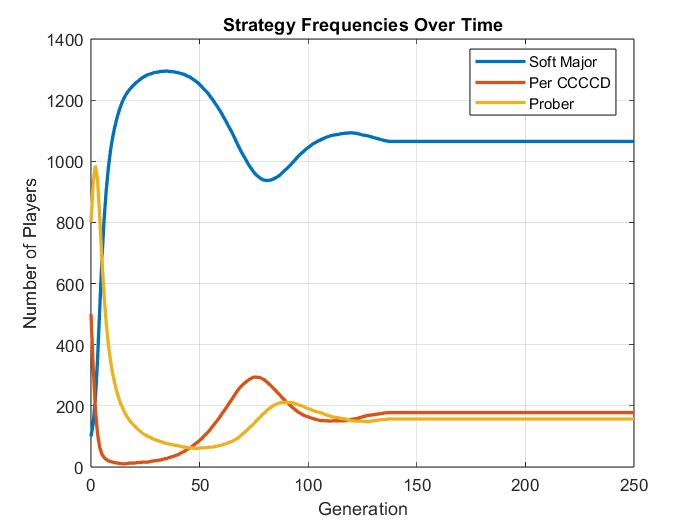
\includegraphics[width=0.7\linewidth]{fit_plots_simulations/disordered_oscillations_sim}
\caption{\texttt{disordered\_oscillations\_sim.m}}
\label{fig:disorderedoscillationssim}
\end{figure}

Παρατηρούμε παρόμοια συμπεριφορά με τη θεωρητική ανάλυση, ωστόσο οι μεταβολές είναι μικρότερες και καταλήγει σε λιγότερες γενιές σε steady state.
\subsubsection{Sensitivity of dynamics to population size}
% TODO: \usepackage{graphicx} required
\begin{figure}[ht!]
\centering
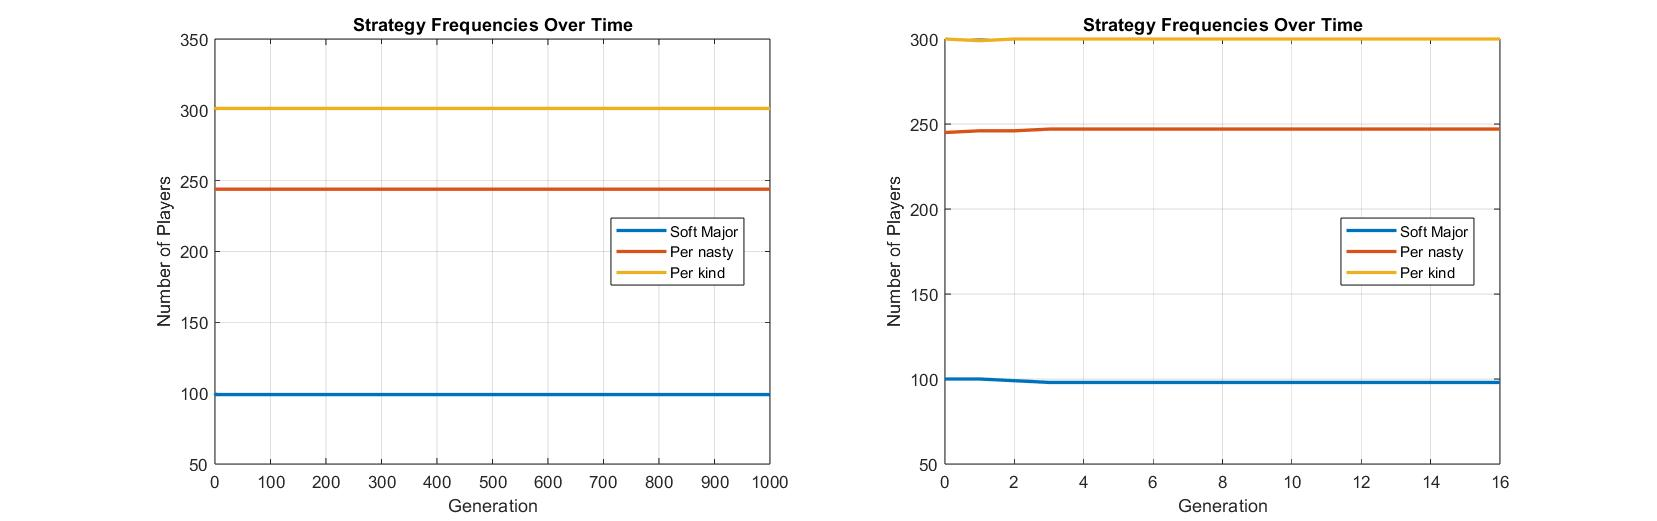
\includegraphics[width=1\linewidth]{fit_plots_simulations/sensitivity_to_population_size_sim}
\caption{\texttt{sens\_dyn\_pop\_size\_sim.m}}
\label{fig:sensitivitytopopulationsizesim}
\end{figure}

Παρατηρούμε ότι οι αρχικές συνθήκες που στην θεωρητική ανάλυση προκαλούν περιοδικές ταλαντώσεις στην προσομοίωση αποτελούν ήδη steady state.\clearpage
\subsubsection{Sensitivity of dynamics to winner}
% TODO: \usepackage{graphicx} required
\begin{figure}[th!]
\centering
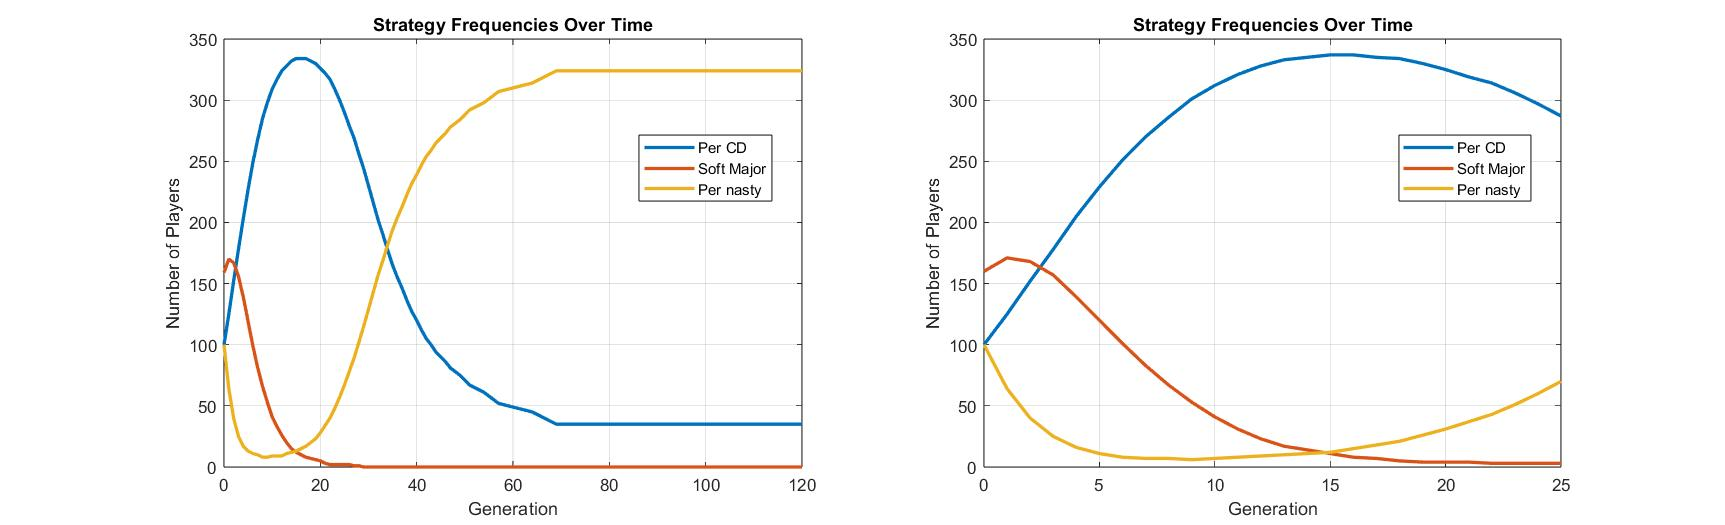
\includegraphics[width=1\linewidth]{fit_plots_simulations/sensitivity_of_winner_to_popsize_sim}
\caption{\texttt{sens\_win\_pop\_size\_sim.m}}
\label{fig:sensitivityofwinnertopopsizesim}
\end{figure}

Παρατηρούμε παρόμοια συμπεριφορά με τη θεωρητική ανάλυση

\subsubsection{Sensitivity to CIPD Payoff}




% TODO: \usepackage{graphicx} required
\begin{figure}[th!]
\centering
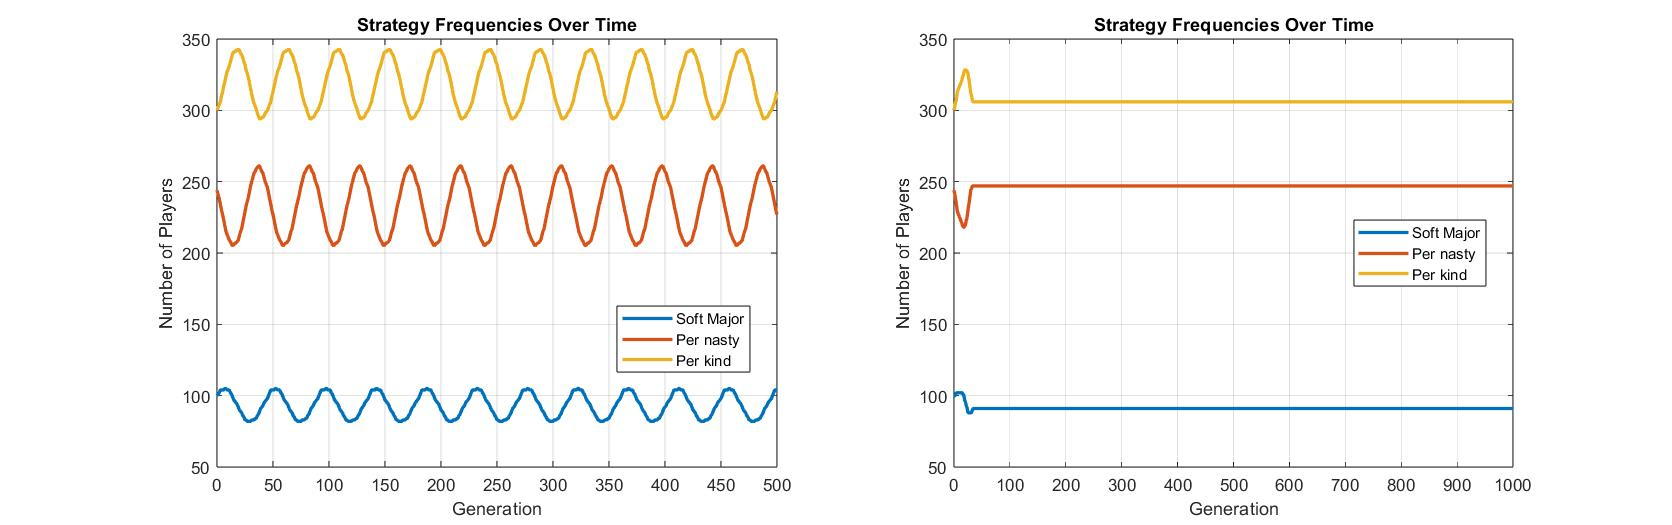
\includegraphics[width=1\linewidth]{fit_plots_simulations/sensitivity_to_cipd_payoff_sim}
\caption{\texttt{sens\_cipd\_payoff\_sim.m}}
\label{fig:sensitivitytocipdpayoffsim}
\end{figure}
Παρατηρούμε στη θεωρητική ανάλυση ότι με τις τιμές αυτές του πίνακα των σκορ έχουμε αυξανόμενες ταλαντώσεις και περιοδικές ταλαντώσεις ενώ στην προσομοίωση αντίστοιχα περιοδικές ταλαντώσεις και ένα σύντομο μεταβατικό φαινόμενο που οδηγεί σε steady state. 
\subsubsection{Sensitivity to Game Length}
% TODO: \usepackage{graphicx} required
\begin{figure}[th!]
\centering
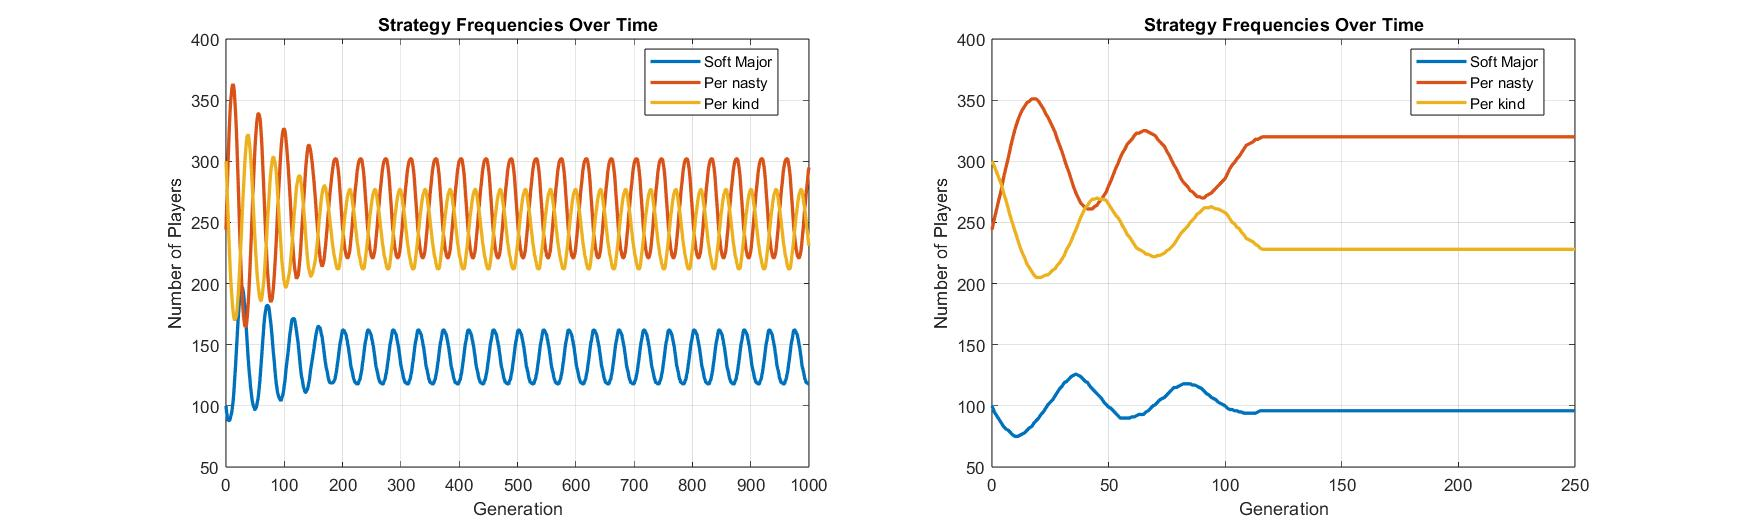
\includegraphics[width=1\linewidth]{fit_plots_simulations/sensitivity_to_game_length_sim}
\caption{\texttt{sens\_game\_length\_sim.m}}
\label{fig:sensitivitytogamelengthsim}
\end{figure}

Παρατηρούμε παρόμοια συμπεριφορά με τη θεωρητική ανάλυση

\subsubsection{Repartition divided by 10}
% TODO: \usepackage{graphicx} required
\begin{figure}[th!]
\centering
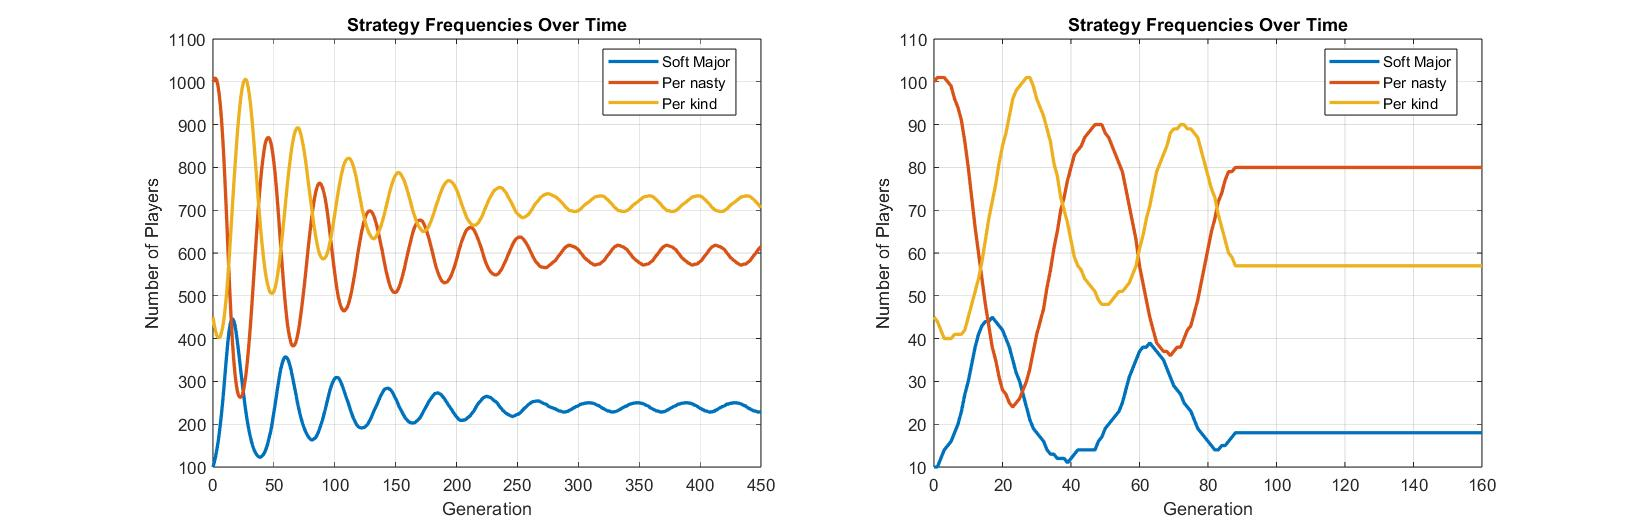
\includegraphics[width=0.7\linewidth]{fit_plots_simulations/repartition_div10_sim}
\caption{\texttt{sens\_repartition\_div10\_sim.m}}
\label{fig:repartitiondiv10sim}
\end{figure}

Παρατηρούμε πως ενώ στη θεωρητική ανάλυση είχαμε μειούμενες και αυξανόμενες ταλαντώσεις στην προσομοίωση έχουμε και στις δύο περιπτώσεις μειούμενες ταλαντώσεις οι οποίες όμως στην περίπτωση της διαίρεσης  με το 10 των πληθυσμών ανατρέπουν και την κατάταξη των στρατηγικών.




